%% Journal of Econometrics submission, Elsevier elsarticle (Harvard/authoryear).
%% Template: elsarticle-template-harv.tex (elsarticle 3.x).
\documentclass[preprint,12pt,authoryear,times]{elsarticle}

\usepackage{amssymb,mathtools,amsthm,booktabs,float,siunitx}
\usepackage[hidelinks]{hyperref}
\mathtoolsset{showonlyrefs}

\journal{Journal of Econometrics}

\newtheorem{theorem}{Theorem}
\newtheorem{remark}{Remark}

\newcommand{\E}{\mathbb{E}}
\newcommand{\Q}{\mathbb{Q}}
\newcommand{\R}{\mathbb{R}}

\begin{document}

\begin{frontmatter}

\title{Identifying Risk-Neutral Densities from an Empirical Measure of Listed Quotes}

\author[ifz]{Simon A.\ Broda\corref{cor1}}
\ead{simon.broda@hslu.ch}
\affiliation[ifz]{organization={Institute of Financial Services IFZ, Lucerne University of Applied Sciences},
            addressline={Suurstoffi 1},
            city={Rotkreuz},
            postcode={6343},
            country={Switzerland}}
\cortext[cor1]{Corresponding author.}

\begin{abstract}
European option prices of a single maturity encode the risk-neutral density of the underlying at expiry. Differentiating those prices twice is ill-posed on a finite strike list. This paper rescales the calls to a complementary distribution function and smooths the jump measure of that function with a Gaussian kernel. The density estimator is minus the forward times the derivative of the resulting kernel density, one term per strike. The kernel cdf of the same measure is a call interpolant. Completing the unquoted tails, placing masses at cell centers, and combining two kernel widths are quadrature corrections. Inside a filling strike grid the estimator is uniformly consistent for exact quotes. Over the whole line the signed estimator integrates to zero and its first moment equals the forward. On exact Heston quotes the density formula brings the integrated squared error to \(5.0\times 10^{-9}\). Prices are never obtained by integrating that formula. They are read from the kernel cdf. Section~\ref{sec:noise} scores the density. Section~\ref{sec:emp} scores the interpolant on listed slices. Under noise the calls are projected onto the decreasing convex cone and the wings are held at the wing implied volatility before either readout.
\end{abstract}

\begin{keyword}
risk-neutral density \sep option prices \sep kernel estimation \sep in-fill consistency \sep state-price density
\MSC[2010] 62G07 \sep 62G20 \sep 62P05 \sep 91G20
\JEL C14 \sep C58 \sep G13
\end{keyword}

\end{frontmatter}

\section{Introduction}
\label{sec:intro}

\citet{breeden1978} identified the risk-neutral density of the underlying at a fixed expiry with the second strike derivative of the corresponding European call, scaled by a discount factor. The identity assumes a twice differentiable price curve. A market supplies a finite ordered list of strikes and a quote at each knot. Numerical second differentiation of that list is ill-posed: interpolants oscillate, change sign, and depend on the interpolating scheme. The literature responds with parametric mixtures and Gram--Charlier expansions, implied-volatility interpolants, local polynomials of the call, and \citet{bondarenko2003}'s positive convolution approximation, which forces the density to be a mixture of a positive kernel with a discrete probability fitted to prices. Section~\ref{sec:lit} reviews these approaches.

This paper estimates the density from a single-maturity strip by rescaling the calls to a complementary distribution function, replacing the empirical jump measure by a Gaussian kernel, and inverting the associated characteristic function. For a Gaussian the inversion is a finite sum, one term per strike. Completing the unquoted tails, placing each mass at the center of its cell, and combining two kernel widths are quadrature corrections. As the strike mesh fills a compact interval and the bandwidth shrinks more slowly than the mesh, the estimator converges to the true density on the interior of that interval.

The usual split in this literature is that interpolants of the call or of implied volatility reprice listed quotes well and do not yield a usable density, while methods that are densities by construction cannot interpolate a dense, slightly arbitrageable chain. \citeauthor{bondarenko2003}'s method is a sieve: with a kernel width that does not shrink as strikes are added, it does not become a local smoother, and it is a density by construction. \citet{yatchew2006} replace the quoted calls by a decreasing convex list; at a zero roughness penalty the second differences of that list are a discrete nonnegative measure, not a curve. \citet{aitsahalia2003} smooth the same constrained list with a local polynomial, so the density is nonnegative by design and the call cannot match quotes that violate convexity. The estimator returns two readouts of one kernel. The density formula is \(-\,F\) times the derivative of the kernel density of the jumps. The call interpolant is the kernel cdf, clipped to \([0,1]\). Over the whole line the signed density integrates to zero and its first moment equals the forward, so the prices are not integrals of \(\hat f_{\Q}\). Section~\ref{sec:noise} scores the density formula on noisy Heston and variance-gamma draws, against the constrained local polynomial, the convolution, and an SVI slice \citep{gatheral2006,gatheraljacquier2014}. Section~\ref{sec:emp} scores the interpolant on four listed slices. Under noise the calls are projected and the wings are filled at constant implied volatility before either readout. On the listed slices the unsmoothed projection remains the closest call. It does not return a density. 

The remainder of this manuscript is structured as follows. Section~\ref{sec:lit} reviews related work. Section~\ref{sec:est} derives the characteristic function of the normalized call and the closed-form estimator, and compares it to kernel smoothing of the call. Section~\ref{sec:refine} records the quadrature corrections and the integral identities. Section~\ref{sec:h} chooses the bandwidth. Section~\ref{sec:ifc} proves in-fill consistency and illustrates it on exact Heston and variance-gamma quotes. Section~\ref{sec:noise} repeats the comparison on irregular strikes with noise in implied volatility, against retuned benchmarks and an SVI slice. Section~\ref{sec:emp} is an illustration on four listed chains from three snapshots. Section~\ref{sec:conc} concludes.

\section{Related Work}
\label{sec:lit}

The identity of Section~\ref{sec:est} is the continuous-strike version of a spanning argument of \citet{ross1976}: if one could trade a put at every strike, the second derivative of the put curve would be a density, and one could synthesize any sufficiently regular payoff. \citet{dupire1994} obtained the analogous result in calendar time, which produces a local-volatility equation. Observed markets supply neither a continuum of strikes nor noiseless quotes.

A first family of methods specifies the density of \(S_T\) as a parametric curve and fits the implied option prices to the quotes. \citet{ritchey1990} and \citet{melick1997} take the density to be a mixture of lognormals, so that the call price is a mixture of Black--Scholes prices; \citet{bahra1997} and \citet{soderlind1997} use related specifications for interest-rate and foreign-exchange options. Two or three components typically suffice to generate a unimodal, skewed density, but the fit is poorly identified once more than two components are admitted, and the approximation to a Heston or jump-diffusion density need not vanish as more quotes arrive. Expansion methods perturb a baseline density---usually lognormal---by Gram--Charlier or Hermite terms \citep{jarrowrudd1982,corradosu1996,rompolis2007,xiu2014}. The expansions can match a finite number of moments, but they are not guaranteed to stay nonnegative, and the truncated series can oscillate in the tails.

A second, and in applied work the most common, family interpolates the Black--Scholes implied-volatility function of strike and converts the interpolant back to prices before differentiating twice. \citet{shimko1993} fitted a quadratic in strike; \citet{malz1997} used a cubic spline in delta; \citet{bliss2002} a smoothing spline. \citet{figlewski2010} completes the tails with a generalized extreme-value distribution. Because implied volatility is a much flatter function of strike than the call itself, a low-order interpolant often has small bias when quotes are accurate. The drawback is that implied volatility is a nonlinear transformation that inflates price noise where the derivative of price with respect to implied volatility is small, i.e.\ in the tails. An interpolating spline then treats those noisy tail quotes as exact, and the second derivative of the resulting call curve oscillates and can become negative. Shape-constrained smoothers of the implied-volatility surface \citep{fengler2005,fengler2009,gatheraljacquier2014,ludwig2015} address the sign problem at the cost of a more involved optimization.

A third family estimates the call as a function of strike by kernel regression or local polynomials and obtains the second derivative from the fit. \citet{priestley1972} fitted a kernel to observed function values at the design points; the risk-neutral density is obtained by differentiating that fit twice. \citet{aitsahalia1998} estimated the call as a function of \((S,K,T,r,q)\) by kernel regression; \citet{aitsahalia2000} used the estimator to recover an implied risk-aversion function. The method is data intensive and, in the original application, pooled option prices across many trading dates. \citet{aitsahalia2003} developed a local polynomial estimator that imposes monotonicity and convexity of \(C\) in \(K\), hence nonnegativity of the density. Related constrained least-squares estimators are studied by \citet{yatchew2006} and \citet{birke2009}; \citet{grith2012} survey the kernel literature. \citet{fanmancini2009} combine a parametric guide with a nonparametric correction. In each case the density is the second strike derivative of a smoother of \(C\). The estimator of Section~\ref{sec:est} rescales the calls to a complementary cumulative distribution function (cdf) and applies the kernel to the empirical jump measure, so the formula is a first derivative of a Gaussian kernel density and is a finite sum. Section~\ref{sec:naive} records the comparison. Sections~\ref{sec:noise} and~\ref{sec:emp} implement the cubic \citeauthor{priestley1972} estimator of that section and the two-step procedure of \citeauthor{aitsahalia2003}: a least-squares projection of the quoted calls onto the decreasing convex cone, followed by a local polynomial of the constrained values. The pricing bandwidth of each is chosen by even/odd cross-validation. The local-cubic bandwidth keeps the second-derivative rate \(n^{-1/9}\).

\citet{bondarenko2003} proposed the positive convolution approximation (PCA). The density is required to lie in the set of functions obtained by convolving a discrete probability with a positive kernel, and the discrete probability is chosen to minimize the sum of squared pricing errors. The kernel enforces smoothness and, together with positive weights, guarantees that the result is a density. In \citeauthor{bondarenko2003}'s comparison, the method dominated mixtures of lognormals, Hermite expansions, and several regularization methods. Subsequent simulation evidence on affine jump-diffusions is consistent with this ranking \citep{lu2019}. Sections~\ref{sec:noise} and~\ref{sec:emp} implement a log-price analog: forty-one lognormal components with a common width, centered on a uniform grid in log strike from the first quoted strike to the last, fitted by nonnegative least squares. Sum-to-one and forward-mean penalties are left as penalties. The weights are not rescaled after the fit, and the width is chosen by even/odd cross-validation, with the grid starting at the center spacing. The same sections choose the roughness penalty of \citeauthor{yatchew2006} by the same cross-validation. Zero is on the grid, so the interpolating projection remains available.

\citet{rubinstein1994} and \citet{jackwerth1996} recovered probabilities on a binomial tree by minimizing a distance to a prior subject to pricing constraints. \citet{stutzer1996} and \citet{buchen1996} maximized entropy. These methods produce a valid density by construction, but the finite-support discretization and the choice of prior affect the tails. Viewing the problem as a linear inverse problem, \citet{cont2004} calibrated jump-diffusion models under a relative-entropy penalty; \citet{monnier2014} used the singular value decomposition of a restricted put operator.

A number of papers compare methods on market data, where the true density is unknown, so that the criterion is typically pricing error or stability over time \citep{cooper1999,jondeau2000,coutant2001,anagnou2005,bliss2002,liu2007}. Studies that generate options from a known process are less common. \citet{bondarenko2003} finds that his method outperforms mixtures, expansions, and several regularization methods on integrated squared error. \citet{lai2014} finds that kernel regression outperforms spline interpolation and neural nets on pricing error. \citet{santos2015} compare mixtures, Edgeworth expansions, hypergeometric functions, and a \citeauthor{bliss2002} smoothing spline against Heston and other targets. \citet{lu2019} compares methods on affine jump-diffusions and again finds \citeauthor{bondarenko2003}'s method accurate. The typical ranking is that implied-volatility interpolants price well when quotes are clean, that mixtures are unstable once more than two components are admitted, and that \citeauthor{bondarenko2003}'s method is the most accurate among methods that do not use a parametric density of \(S_T\), when the true density is known. Section~\ref{sec:ifc} is in this vein for exact quotes: the targets are Heston and variance-gamma, and only the nested versions of the estimator in this paper are scored. Section~\ref{sec:noise} puts the same targets behind an irregular strike grid and one volatility point of noise, and scores the retuned benchmarks on integrated squared error. Section~\ref{sec:emp} scores four listed slices, where the true density is unknown, on pricing error.

\section{Construction of the Estimator}
\label{sec:est}

\subsection{Construction}
\label{sec:construct}

Assume a risk-neutral measure \(\Q\) under which \(S_T\) has a density \(f_{\Q}\) on \((0,\infty)\) and \(\E^{\Q}[S_T]<\infty\). Let \(r\) be the continuously compounded interest rate and \(q\) the continuous dividend yield. Write \(F=S_0e^{(r-q)T}\) for the forward. Under \(\Q\),
\begin{align}
S_0e^{-qT}
&\;=\;
e^{-rT}\,\E^{\Q}[S_T]
\nonumber\\
&\;=\;
e^{-rT}\int_{0}^{\infty}x\,f_{\Q}(x)\,\mathrm{d}x,
\label{eq:S0}
\end{align}
hence \(\E^{\Q}[S_T]=F\). Write \(C\) for the corresponding call curve:
\begin{align}
C(K)
&\;=\;
e^{-rT}\,\E^{\Q}\bigl[(S_T-K)^+\bigr]
\nonumber\\
&\;=\;
e^{-rT}\int_K^{\infty}(x-K)\,f_{\Q}(x)\,\mathrm{d}x.
\label{eq:C}
\end{align}
Now define the normalized option price
\begin{equation}
\label{eq:Ctil}
\tilde C(K)
\;\equiv\;
\frac{C(K)}{S_0e^{-qT}}
\;=\;
\frac{\displaystyle\int_K^{\infty}(x-K)\,f_{\Q}(x)\,\mathrm{d}x}{F}.
\end{equation}

The normalized call price is a decreasing function of \(K\): it is equal to \(1\) if \(K=0\) and equal to \(0\) if \(K=\infty\). Thus the normalized call price, as a function of \(K\), is a complementary cdf, say \(\tilde C(K)=1-P(K)\). The characteristic function (hereafter c.f.) of the law of \(P\) is the Fourier--Stieltjes transform
\begin{equation}
\label{eq:phi-P-stieltjes}
\varphi_P(s)
\;=\;
\int_{(0,\infty)}e^{\mathrm{i}s K}\,\mathrm{d}P(K).
\end{equation}
For a cdf on \([0,\infty)\) and \(s\neq 0\), \eqref{eq:phi-P-stieltjes} is
\begin{equation}
\varphi_P(s)
\;=\;
1+\mathrm{i}s\int_0^{\infty}e^{\mathrm{i}s K}\,\tilde C(K)\,\mathrm{d}K.
\end{equation}
Substitute \eqref{eq:Ctil}. Fubini yields
\[
\int_0^{\infty}e^{\mathrm{i}s K}\,\tilde C(K)\,\mathrm{d}K
\;=\;
\frac{1}{F}\int_0^{\infty}f_{\Q}(x)\Biggl[\int_0^x e^{\mathrm{i}s K}(x-K)\,\mathrm{d}K\Biggr]\mathrm{d}x.
\]
The inner integral is \(-x/(\mathrm{i}s)+(e^{\mathrm{i}s x}-1)/(\mathrm{i}s)^2\). Hence, for \(s\neq 0\),
\begin{align}
\varphi_P(s)
&\;=\;
1+\frac{\mathrm{i}s}{F}\int_0^{\infty}f_{\Q}(x)\Biggl[-\frac{x}{\mathrm{i}s}+\frac{e^{\mathrm{i}s x}-1}{(\mathrm{i}s)^2}\Biggr]\mathrm{d}x
\nonumber\\
&\;=\;
1-F^{-1}\E^{\Q}[S_T]+\frac{\varphi_{\Q}(s)-1}{\mathrm{i}s\,F}
\nonumber\\
&\;=\;
\frac{\varphi_{\Q}(s)-1}{\mathrm{i}s\,F},
\label{eq:phi-P}
\end{align}
where \(\varphi_{\Q}(s)=\E^{\Q}[e^{\mathrm{i}s S_T}]\) and \(\E^{\Q}[S_T]=F\) by \eqref{eq:S0}. Solving for \(\varphi_{\Q}\), one obtains
\begin{equation}
\label{eq:phi-Q}
\varphi_{\Q}(s)
\;=\;
1+\mathrm{i}s\,F\,\varphi_P(s).
\end{equation}
Read from the right, \eqref{eq:phi-P} is a pricing formula: a model that supplies \(\varphi_{\Q}\) yields \(\varphi_P\), hence the complementary cdf \(\tilde C=1-P\) and the call \citep{lewis2000}. This paper inverts the identity: \(\varphi_P\) is constructed from the quotes, and \(\varphi_{\Q}\) is recovered.

The c.f.\ \(\varphi_{\Q}\) is that of \(S_T\). Fourier inversion yields
\begin{equation}
\label{eq:f-Q}
f_{\Q}(K)
\;=\;
\frac{1}{2\pi}\int_{-\infty}^{\infty}e^{-\mathrm{i}s K}\,\varphi_{\Q}(s)\,\mathrm{d}s.
\end{equation}
Substitute \eqref{eq:phi-Q} into \eqref{eq:f-Q}:
\begin{equation}
\label{eq:f-Q-plug}
f_{\Q}(K)
\;=\;
\frac{1}{2\pi}\int_{-\infty}^{\infty}e^{-\mathrm{i}s K}\,\mathrm{d}s
+\frac{F}{2\pi}\int_{-\infty}^{\infty}e^{-\mathrm{i}s K}\,(\mathrm{i}s)\,\varphi_P(s)\,\mathrm{d}s.
\end{equation}
The first integral is a Dirac mass at \(K=0\). For \(K>0\),
\begin{equation}
\label{eq:f-Q-pos}
f_{\Q}(K)
\;=\;
\frac{F}{2\pi}\int_{-\infty}^{\infty}e^{-\mathrm{i}s K}\,(\mathrm{i}s)\,\varphi_P(s)\,\mathrm{d}s.
\end{equation}

Observed calls at strikes \(0<K_1<\cdots<K_m\) supply an empirical complementary cdf \(\tilde C_i=C_i/(S_0e^{-qT})\) and hence an empirical cdf \(P_i=1-\tilde C_i\). Write
\begin{equation}
\label{eq:nu}
\nu_m
\;=\;
\sum_{i=1}^m\Delta P_i\,\delta_{K_i},
\qquad
\Delta P_i
\;=\;
P_i-P_{i-1},
\quad
P_0:=0.
\end{equation}
The c\`adl\`ag interpolant of these knots is a step function \(P_m\). Its Fourier--Stieltjes transform is the finite sum \(\int e^{\mathrm{i}s K}\,\mathrm{d}P_m(K)=\sum_i\Delta P_i e^{\mathrm{i}s K_i}\), which is also the c.f.\ of \(\nu_m\). Replace \(\varphi_P\) by the product of that sum with the Fourier transform of a Gaussian kernel of width \(h\),
\begin{equation}
\label{eq:phi-hat}
\hat\varphi_P(s)
\;=\;
\Biggl(\sum_{i=1}^m\Delta P_i e^{\mathrm{i}s K_i}\Biggr)e^{-h^2 s^2/2}.
\end{equation}
Formally, the estimator is \eqref{eq:f-Q-pos} with \(\varphi_P\) replaced by \(\hat\varphi_P\):
\begin{equation}
\label{eq:fhat-Q-ft}
\hat f_{\Q}(K)
\;=\;
\frac{F}{2\pi}\int_{-\infty}^{\infty}e^{-\mathrm{i}s K}\,(\mathrm{i}s)\Biggl(\sum_{i=1}^m\Delta P_i e^{\mathrm{i}s K_i}\Biggr)e^{-h^2 s^2/2}\,\mathrm{d}s.
\end{equation}
The integrand is a finite sum. The Fourier transform of \(e^{\mathrm{i}s K_i}e^{-h^2 s^2/2}\) is the \(N(K_i,h^2)\) density
\begin{equation}
\label{eq:kappa}
\kappa_h(u)
\;=\;
\frac{1}{h\sqrt{2\pi}}\,\exp\Bigl(-\frac{u^2}{2h^2}\Bigr),
\end{equation}
and multiplication by \(\mathrm{i}s\) is differentiation up to sign: if \(\varphi(s)=\int e^{\mathrm{i}s u}\kappa_h(u-K_i)\,\mathrm{d}u\), then the transform of \(\kappa_h'(\,\cdot\,-K_i)\) is \(-\mathrm{i}s\,\varphi(s)\), so the transform of \(\mathrm{i}s\,\varphi(s)\) is \(-\kappa_h'(\,\cdot\,-K_i)\). Therefore
\begin{equation}
\label{eq:fhat-Q}
\hat f_{\Q}(K)
\;=\;
-F\sum_{i=1}^m\Delta P_i\,\kappa_h'(K-K_i)
\;=\;
F\sum_{i=1}^m\Delta P_i\,\frac{K-K_i}{h^2}\,\kappa_h(K-K_i),
\end{equation}
where \(\kappa_h'(u)=-(u/h^2)\kappa_h(u)\). Equation \eqref{eq:fhat-Q} is a closed-form sum. It is \(-F\) times the first derivative of the Gaussian kernel density of \(\nu_m\). The kernel density itself is a Gaussian mixture. The estimator of \(f_{\Q}\) is not: each term is a Gaussian density multiplied by \((K-K_i)/h^2\). The interpolant of the complementary-call cdf is the kernel cdf of the same measure, and that interpolant does not differentiate the kernel. Let \(\mathcal{K}\) denote the standard Gaussian cdf. Then
\begin{equation}
\label{eq:P-hat}
\hat P(K)
\;=\;
\sum_{i=1}^m\Delta P_i\,\mathcal{K}\bigl((K-K_i)/h\bigr),
\end{equation}
and calls are \(\hat C=S_0e^{-qT}(1-\hat P)\). Differentiating \(\hat P\) twice and multiplying by \(-F\) recovers \eqref{eq:fhat-Q}.
\label{sec:closed}

\subsection{Comparison to Naive Kernel Smoothing}
\label{sec:naive}

In the continuum, \citeauthor{breeden1978} plus a kernel is unambiguous. If \(C\) is the true call curve,
\begin{equation}
\label{eq:smooth-C}
(C\ast\kappa_h)''
\;=\;
C''\ast\kappa_h
\;=\;
e^{-rT}\,(f_{\Q}\ast\kappa_h).
\end{equation}
Smoothing \(C\) and differentiating twice is a kernel smooth of \(f_{\Q}\). On a strike list the discretization matters.

A \citeauthor{priestley1972} estimator treats the observations as levels \(C_i\) and weights them by the design spacing \(\Delta K_i=K_i-K_{i-1}\) (\(K_0:=K_1-(K_2-K_1)\)):
\begin{equation}
\label{eq:pc}
\hat C^{\mathrm{PC}}(K)
\;=\;
\sum_{i=1}^m\Delta K_i\,C_i\,\kappa_h(K-K_i),
\qquad
\hat f_{\Q}^{\mathrm{PC}}(K)
\;=\;
e^{rT}\sum_{i=1}^m\Delta K_i\,C_i\,\kappa_h''(K-K_i),
\end{equation}
where \(\kappa_h''(u)=(u^2/h^2-1)h^{-2}\kappa_h(u)\). The equivalent kernel for the density is \(\kappa''\). The interpolant is a mixture of the prices.

That sum is a Riemann approximation to \eqref{eq:smooth-C}. It treats the observed levels as atoms of a measure. They are not: \(C\) is a smooth function of \(K\), observed at the knots. Convolution requires a function on the line. A linear interpolant of \(C\) has second derivative zero almost everywhere and Dirac masses at the kinks, so it cannot recover \(f_{\Q}\). The usual construction is a cubic spline \(C^{\mathrm{cs}}\) through the quotes, extended by linear wings of slope in \([-e^{-rT},0]\):
\begin{equation}
\label{eq:pc-cubic}
\hat f_{\Q}^{\mathrm{cs}}(K)
\;=\;
e^{rT}\,(C^{\mathrm{cs}}\ast\kappa_h)''(K).
\end{equation}
A cubic is the lowest-degree interpolant whose second derivative is not identically zero on each cell; the same degree appears in local-polynomial estimation of a second derivative \citep{aitsahalia2003}. Without the interpolant, \eqref{eq:pc} places a large weight on \(\kappa''\) wherever \(C\) is large, including deep in the money where \(C\) is nearly linear and \(C''\) is nearly zero.

Equation \eqref{eq:fhat-Q} does not need a spline. The object being smoothed is already a discrete measure, \(\nu_m=\sum_i\Delta P_i\,\delta_{K_i}\). Convolution with \(\kappa_h\) is the finite mixture \(\sum_i\Delta P_i\,\kappa_h(\,\cdot\,-K_i)\), and one derivative of that mixture is \eqref{eq:fhat-Q}. The c\`adl\`ag interpolant of \(P\) is a step function; smoothing a step function is kernel density estimation, not kernel regression of a curve.

On an equal grid with already monotone \(C\), \(\Delta C_i\approx C'(K_i)\delta\), so \eqref{eq:pc} and \eqref{eq:fhat-Q} are close. They are not close when \(C\) is large and locally linear, as a deep in-the-money call is. Section~\ref{sec:emp} implements the cubic interpolant \eqref{eq:pc-cubic} on listed chains.

\section{Three Refinements}
\label{sec:refine}

\subsection{Completing the Tails}
\label{sec:tails}

The empirical measure \eqref{eq:nu} puts mass \(P(K_1)\) at the first quoted strike and mass \(1-P(K_m)\) nowhere. Both ends are wrong as a cdf on \((0,\infty)\).

On \((0,K_1]\) a deep in-the-money call is intrinsic, \(C(K)=e^{-rT}(F-K)\), hence \(\tilde C(K)=1-K/F\) and \(P(K)=K/F\). That is a straight line through the origin. The estimator matches the observed \(P(K_1)\) rather than \(K_1/F\),
\begin{equation}
\label{eq:left}
P(K)
\;=\;
P(K_1)\,\frac{K}{K_1},
\qquad
0<K\le K_1.
\end{equation}
When the first quote is at intrinsic, \(P(K_1)=K_1/F\) and \eqref{eq:left} is exactly \(K/F\). The line is replaced by \(n_L=\mathrm{round}(K_1/\delta)\) equal jumps of size \(P(K_1)/n_L\) on a uniform grid of \((0,K_1]\), where \(\delta\) is the median quoted gap, and the original jump \(\Delta P_1=P(K_1)\) at \(K_1\) is removed. That choice continues the quoted mesh through the splice at \(K_1\).

On the right, \(\tilde C(\infty)=0\) so \(P(\infty)=1\). If \(C_m>0\), a European call still has to fall to zero. The residual call is continued linearly with slope in \([-e^{-rT},0)\) until \(C=0\) at an intercept \(K_{\mathrm{end}}\). That wing is a line. The last listed gap is much coarser than \(\delta\), so the knots are a quadrature of the line rather than a continuation of the quoted mesh. Eight knots per last gap,
\begin{equation}
\label{eq:nR}
n_R
\;=\;
\mathrm{round}\bigl(8(K_{\mathrm{end}}-K_m)/(K_m-K_{m-1})\bigr),
\end{equation}
are equally spaced in \((K_m,K_{\mathrm{end}}]\) and converted to \(P=1-\tilde C\). If \(C_m=0\), \(P(K_m)=1\) already and this wing is empty.

Only the left completion changes the estimator on the Heston and variance-gamma chains below: the first quoted call is at intrinsic, and the last quoted call is already zero (dense) or of order \(10^{-5}\) (sparse).

\subsection{Midpoint Rule}
\label{sec:mid}

Placing each jump \(\Delta P_i\) at the right endpoint of its cell \((K_{i-1},K_i]\) is a rectangle rule for the Stieltjes integral against \(P\). The midpoint rule puts the same mass at the cell center. Write \(K_0:=0\) and
\begin{equation}
\label{eq:mid}
\tilde K_j
\;=\;
\tfrac12\bigl(K_{j-1}^{\ast}+K_j^{\ast}\bigr),
\end{equation}
where \(K_1^{\ast}<\cdots<K_N^{\ast}\) is the completed strike list. For a Gaussian integrand on an equally spaced grid the midpoint error is smaller than any power of \(\delta/h\). Combined with both tails,
\begin{equation}
\label{eq:headline}
\hat f_{\Q}(K)
\;=\;
F\sum_{j=1}^{N}\Delta_j\,\frac{K-\tilde K_j}{h^2}\,\kappa_h(K-\tilde K_j),
\end{equation}
with \(\kappa_h\) as in \eqref{eq:kappa} and \(\Delta_j\) the jump on \((K_{j-1}^{\ast},K_j^{\ast}]\). Equation \eqref{eq:fhat-Q} is the same sum with \(\tilde K_j\) replaced by the right endpoints \(K_j^{\ast}\). The interpolant on that support is \eqref{eq:P-hat} with each \(K_i\) replaced by \(\tilde K_j\),
\begin{equation}
\label{eq:P-hat-mid}
\hat P(K)
\;=\;
\sum_{j=1}^{N}\Delta_j\,\mathcal{K}\bigl((K-\tilde K_j)/h\bigr).
\end{equation}

\subsection{Twicing}
\label{sec:twice}

The Gaussian kernel in \eqref{eq:headline} has second moment \(h^2\), so the leading bias of \(\hat f_{\Q}\) is \(O(h^2)\). When the quotes are treated as exact there is no observation-error variance to inflate, and a higher-order kernel is admissible. Twicing \citep{schucanysommers1977} replaces the kernel transform \(e^{-h^2 s^2/2}\) in \eqref{eq:phi-hat} by
\begin{equation}
\label{eq:phi-twice}
2e^{-h^2 s^2/2}-e^{-h^2 s^2},
\end{equation}
which is the Fourier transform of \(2\kappa_h-\kappa_{h\sqrt{2}}\). The equivalent kernel has vanishing second moment, so the \(O(h^2)\) bias becomes \(O(h^4)\). In closed form,
\begin{equation}
\label{eq:twice}
\hat f_{\Q}^{\mathrm{tw}}(K)
\;=\;
2\hat f_{\Q,h}(K)-\hat f_{\Q,h\sqrt{2}}(K),
\end{equation}
and the same combination is applied to the interpolant \eqref{eq:P-hat-mid}, \(\hat P^{\mathrm{tw}}=2\hat P_h-\hat P_{h\sqrt{2}}\). The equivalent kernel takes negative values, so \(\hat f_{\Q}^{\mathrm{tw}}\) is not a density. It is still \(-F\) times the derivative of a two-width Gaussian mixture of the jumps.

Twicing a truncated measure amplifies leakage from the missing tails. It is used only on the completed, midpoint-placed support. Equation \eqref{eq:twice}, applied to \eqref{eq:headline}, is the estimator used below.

\subsection{Integrals}
\label{sec:mass}

The kernel density of the completed midpoint measure, \(m_h=\nu_N\ast\kappa_h\), integrates to \(\sum_j\Delta_j\). When those jumps are the jumps of a cdf the sum equals one, and \(m_h\) is a Gaussian mixture, one component per strike. The density estimator is not the mixture. It is \(\hat f_{\Q}=-F\,m_h'\). Integration by parts, using \(K\,m_h(K)\to 0\) as \(|K|\to\infty\), gives
\begin{equation}
\label{eq:moments}
\int_{-\infty}^{\infty}\hat f_{\Q}(K)\,\mathrm{d}K
\;=\;
0,
\qquad
\int_{-\infty}^{\infty}K\,\hat f_{\Q}(K)\,\mathrm{d}K
\;=\;
F\sum_j\Delta_j.
\end{equation}
The same identities hold after twicing. The kernel \(2\kappa_h-\kappa_{h\sqrt{2}}\) integrates to one, so \(\hat f_{\Q}^{\mathrm{tw}}\) is the derivative of a function that integrates to \(\sum_j\Delta_j\), whether or not that function stays nonnegative. The signed estimator therefore matches the forward and misses the probability. On an exact dense Heston strip, with the mesh bandwidth and twicing, the two integrals on \([-2F,8F]\) equal \(0\) and \(F\) to machine precision, and the positive and negative parts on that window each integrate to about \(1.07\).

Theorem~\ref{thm:ifc} is uniform approximation on compact subsets of an interval \((A,B)\) that the quotes cover. It does not put the missing unit of mass back. The negative part that cancels \(\int_{(A,B)}\hat f_{\Q}\) lies outside that interval, where \(m_h\) is still rising. Call prices below are not integrals of \(\hat f_{\Q}\). They are read from the kernel cdf \(\hat P\), clipped to \([0,1]\). Clipping \(\hat P\) and discarding the negative part of \(\hat f_{\Q}\) are different operations.

\section{Choice of Bandwidth}
\label{sec:h}

The width \(h\) is the only tuning constant in \eqref{eq:twice}. Two rules are used below.

With exact quotes the bias is the usual \(O(h^2)\) kernel bias, or \(O(h^4)\) after twicing, and the remaining discretization error after midpoints is smaller than any power of \(\delta/h\) on an equally spaced Gaussian grid. For a Gaussian it is enough that \(h\) be a small multiple of the typical quoted gap. Write \(\delta\) for the median of \(\{K_i-K_{i-1}\}\) on the quoted strikes, not on the filled wings, and take
\begin{equation}
\label{eq:h-mesh}
h
\;=\;
\min\bigl(1.2\,\delta,\; 0.30\,(K_m-K_1)\bigr).
\end{equation}
The cap binds only on a very short chain. On an equally spaced grid every gap equals \(\delta\). This is the rule in Section~\ref{sec:heston}, where the quotes are exact.

When quotes are noisy, \eqref{eq:h-mesh} inherits the noise in the jumps. A listed chain is a noisy sample of the call curve, not an in-fill of an exact function. The object being smoothed is then closer to a density of the jumps than to a second derivative from a vanishing mesh. Replacing the mesh by the width of \(S_T\) and using the Gaussian exponent of \citet{silverman1986}, \(n^{-1/5}\), yields
\begin{equation}
\label{eq:h-den}
h
\;=\;
1.06\,F\,\hat\sigma_{\mathrm{ATM}}\sqrt{T}\,n^{-1/5},
\end{equation}
where \(\hat\sigma_{\mathrm{ATM}}\) is the at-the-money (ATM) Black--Scholes implied volatility, the median of contracts with \(|K-F|\le 0.03F\) (or the median of all finite implied volatilities if that window is empty), and \(n\) is the number of masses after the right wing of Section~\ref{sec:tails}, not the left filler and not necessarily the number of listed quotes. The scale is the scale of \(S_T\), not the standard deviation of the jumps \(\Delta_j\). The ordinary \citeauthor{silverman1986} rule computed from those jumps oversmooths, because that standard deviation is of the order of the chain width. This is the rule in Section~\ref{sec:emp}.

Theorem~\ref{thm:ifc} requires \(h\to 0\) and \(\delta/h^{3/2}\to 0\) on a general mesh, or \(\delta/h\to 0\) on an equally spaced Gaussian grid. On a sequence of grids that fill a fixed interval with mesh \(\delta\propto n^{-1}\), the density-scale rule has \(h\propto n^{-1/5}\). Then \(h\to 0\) and \(\delta/h^{3/2}=O(n^{-7/10})\to 0\), so \eqref{eq:h-den} satisfies the theorem for exact quotes. The listed chains below are noisy, and the theorem is silent on observation error. The mesh rule keeps \(h/\delta=1.2\), so \(\delta/h\) does not tend to zero and the polynomial midpoint bound \(O(\delta^2/h^3)\) does not vanish. Equation \eqref{eq:h-mesh} is not covered by Theorem~\ref{thm:ifc}. It is a fixed-ratio quadrature for exact, equally spaced quotes, used on the chains of Section~\ref{sec:heston}.

%An even/odd split that interpolates the ecdf \(P\) on even strikes and scores the odd \(P_i\) targets \(P\), not \(P''\), and undersmooths. It is not used as a bandwidth.

\section{In-Fill Consistency}
\label{sec:ifc}

Write \(P\) for the complementary-call cdf of Section~\ref{sec:est}, so that \(f_{\Q}=-F\,P''\) on \((0,\infty)\). The midpoint estimator \eqref{eq:headline} is
\[
\hat f_{\Q}(K)
\;=\;
-F\,(\nu_N\ast\kappa_h)'(K),
\]
where \(\nu_N=\sum_j\Delta_j\delta_{\tilde K_j}\) is the completed, midpoint-placed empirical measure of \(P\).

\begin{theorem}
\label{thm:ifc}
Let \(f_{\Q}\) be four times continuously differentiable on \((0,\infty)\) with \(\E^{\Q}[S_T]<\infty\), and let \(C\) be the corresponding call curve. Fix a compact interval \([A,B]\subset(0,\infty)\). Consider a sequence of exact quote grids \(0<K_1^{(m)}<\cdots<K_m^{(m)}\) with mesh \(\delta_m=\max_i(K_i^{(m)}-K_{i-1}^{(m)})\to 0\), \(K_1^{(m)}\le A\) and \(K_m^{(m)}\ge B\). Complete the tails as in Section~\ref{sec:tails} and place masses at midpoints as in Section~\ref{sec:mid}. Let \(h_m>0\). If \(h_m\to 0\) and \(\delta_m/h_m^{3/2}\to 0\), then both the midpoint estimator \eqref{eq:headline} and its twiced version \eqref{eq:twice} converge to \(f_{\Q}\) uniformly on every compact subset of \((A,B)\). If the grid is equally spaced, the Gaussian Euler--Maclaurin argument of the proof yields the same conclusion under the weaker condition \(\delta_m/h_m\to 0\).
\end{theorem}

\begin{proof}
The midpoint estimator is \(\hat f_{\Q}=-F(\nu_N\ast\kappa_h)'\), and \(f_{\Q}=-F P''\). Split
\[
(\nu_N\ast\kappa_h)'-P''
\;=\;
\bigl((\nu_N-P)\ast\kappa_h'\bigr)
+(P'\ast\kappa_h-P')'.
\]
The second term is ordinary kernel bias of \(P''=-f_{\Q}/F\): \((P'\ast\kappa_h-P')'=(P''\ast\kappa_h)-P''\). Because \(\kappa\) is even, \(\int\kappa=1\) and \(\int u\kappa(u)\,\mathrm{d}u=0\). If \(f_{\Q}''\) is bounded on a neighborhood of \([A,B]\), the difference is \(O(h^2)\) uniformly on compact subsets of \((A,B)\) several bandwidths away from the endpoints. The twiced kernel \(2\kappa_h-\kappa_{h\sqrt{2}}\) has Fourier transform \eqref{eq:phi-twice}, hence vanishing second moment, so the same expansion starts at order \(h^4\) whenever \(f_{\Q}\) is \(C^4\).

The first term is discretization. On each completed cell the midpoint rule integrates \(\kappa_h'(K-\,\cdot\,)\) against \(\mathrm{d}P\). For a \(C^2\) integrand the error on a cell of length at most \(\delta\) is \(O(\delta^3)\) times the second derivative of the integrand. That second derivative is \(O(h^{-4})\) for \(\kappa_h'\), and \(O(h^{-4})\) as well for the twiced equivalent kernel. The kernel window contains \(O(h/\delta)\) cells, so a polynomial bound on the total discretization error is \(O(\delta^2/h^3)\), which vanishes if \(\delta/h^{3/2}\to 0\). For a Gaussian integrand on an equally spaced grid the Euler--Maclaurin formula (the Fourier transform of a Gaussian is a Gaussian) makes the midpoint error smaller than any power of \(\delta/h\), so the weaker condition \(\delta/h\to 0\) already suffices. The c\`adl\`ag placement of Section~\ref{sec:closed}, with masses at the right endpoints, is a rectangle rule. The error on a cell is \(O(\delta^2)\) times the first derivative of the integrand, and that derivative is \(O(h^{-3})\). Over the \(O(h/\delta)\) cells in the kernel window the total is \(O(\delta/h^2)\), which vanishes if \(\delta/h^2\to 0\).

The filled wings are supported on \((0,K_1]\) and, if \(C_m>0\), on \((K_m,K_{\mathrm{end}}]\). Their contribution at an evaluation point \(K\in[A+\varepsilon,B-\varepsilon]\) is at most a constant times \(h^{-2}\exp(-\varepsilon^2/2h^2)\), because \(K_1\le A\) and \(K_m\ge B\). That bound tends to zero faster than any power of \(h\).

Multiplying by \(-F\) yields the claim for \(\hat f_{\Q}\) and for \(\hat f_{\Q}^{\mathrm{tw}}\).
\end{proof}

\begin{remark}
The argument treats quotes as exact. It is not a statement about observation error, and it is not a statement about the far tails outside \([A,B]\). The equivalent kernel of \eqref{eq:twice} takes negative values, so the twiced estimator is not necessarily a density. Equation \eqref{eq:moments} is the complementary global statement: over the whole line the signed estimator integrates to zero.
\end{remark}

\subsection{Numerical Illustration}
\label{sec:heston}

The data-generating process is the stochastic-volatility model of \citet{heston1993} with the equity parameters of \citet{bakshi1997}: \(S_0=100\), \(r=0.05\), \(q=0\), \(T=1/4\), \(\kappa=1.15\), \(\theta=0.04\), \(\sigma=0.39\), \(\rho=-0.64\), \(v_0=0.04\). The c.f.\ of \(\log S_T\) uses the little-trap branch of \citet{albrecher2007}. Call prices are the damped integrand of \citet{carrmadan1999} with damping \(\alpha=1.5\), evaluated by the trapezoid rule on \(4096\) frequencies in \((0,250]\); puts follow by parity. There is no Monte Carlo noise. The true density is Fourier inversion of the same c.f.\ on the same frequency grid,
\begin{equation}
\label{eq:true-q}
f_{\Q}(K)
\;=\;
\frac1{K\pi}\int_0^\infty
\mathrm{Re}\bigl[e^{-\mathrm{i}u\log K}\varphi(u)\bigr]\,\mathrm{d}u,
\end{equation}
where \(\varphi(u)=\E^{\Q}[e^{\mathrm{i}u\log S_T}]\). Two chains are used: a dense grid of \(m=256\) equally spaced strikes on \([30,220]\) (spacing \(\delta=0.745\)) and a sparse grid of \(m=64\) equally spaced strikes on \([70,140]\) (spacing \(\delta=1.11\)). Integrated squared error (ISE) is \(\int_{60}^{150}(\hat f_{\Q}-f_{\Q})^2\,\mathrm{d}K\), evaluated by the trapezoid rule on \(401\) equally spaced points. Table~\ref{tab:heston-tail} reports ISE for the four nested estimators at the oracle \(h^{\ast}\), at the mesh rule \(h=1.2\delta\) of \eqref{eq:h-mesh}, and at the density-scale rule \eqref{eq:h-den}. The oracle minimizes the integral on a geometric grid in \(h\).

\begin{table}[H]
\centering
\caption{Integrated squared error \(\int_{60}^{150}(\hat f_{\Q}-f_{\Q})^2\,\mathrm{d}K\) on exact Heston quotes. Mesh \(h\) is \eqref{eq:h-mesh}. The last pair of columns is \eqref{eq:h-den}. Baseline is \eqref{eq:fhat-Q} on the quoted strikes. Tail completion uses the wings of Section~\ref{sec:tails}. Tail+Midpoint is \eqref{eq:headline}. Tail+Mid+Twice is \eqref{eq:twice}.}
\label{tab:heston-tail}
\resizebox{\textwidth}{!}{%
\begin{tabular}{ll
  S[table-format=2.2]
  S[table-format=1.2e-1, scientific-notation=true]
  S[table-format=2.2]
  S[table-format=1.2e-1, scientific-notation=true]
  S[table-format=2.2]
  S[table-format=1.2e-1, scientific-notation=true]}
\toprule
\multicolumn{1}{c}{Chain} & \multicolumn{1}{c}{Estimator} &
  {\(h^{\ast}\)} & {Oracle ISE} & {Mesh \(h\)} & {Mesh ISE} & {Den.\ \(h\)} & {Den.\ ISE} \\
\midrule
Dense & Baseline \eqref{eq:fhat-Q}
  & 0.63 & 2.67e-5 & 0.89 & 2.71e-5 & 3.41 & 1.45e-4 \\
Dense & Tail completion
  & 0.63 & 2.67e-5 & 0.89 & 2.71e-5 & 3.41 & 1.45e-4 \\
Dense & Tail+Midpoint \eqref{eq:headline}
  & 0.63 & 2.27e-7 & 0.89 & 8.23e-7 & 3.41 & 1.22e-4 \\
Dense & Tail+Mid+Twice \eqref{eq:twice}
  & 0.72 & 3.44e-9 & 0.89 & 5.00e-9 & 3.41 & 8.24e-6 \\
\midrule
Sparse & Baseline \eqref{eq:fhat-Q}
  & 26.83 & 1.07e-2 & 1.33 & 2.87e2 & 4.51 & 7.42e0 \\
Sparse & Tail completion
  & 1.10 & 6.24e-5 & 1.33 & 6.34e-5 & 4.29 & 3.16e-4 \\
Sparse & Tail+Midpoint \eqref{eq:headline}
  & 0.96 & 4.39e-6 & 1.33 & 5.95e-6 & 4.29 & 2.68e-4 \\
Sparse & Tail+Mid+Twice \eqref{eq:twice}
  & 2.14 & 2.07e-6 & 1.33 & 3.24e-6 & 4.29 & 3.09e-5 \\
\bottomrule
\end{tabular}%
}
\end{table}

\begin{figure}[H]
\centering
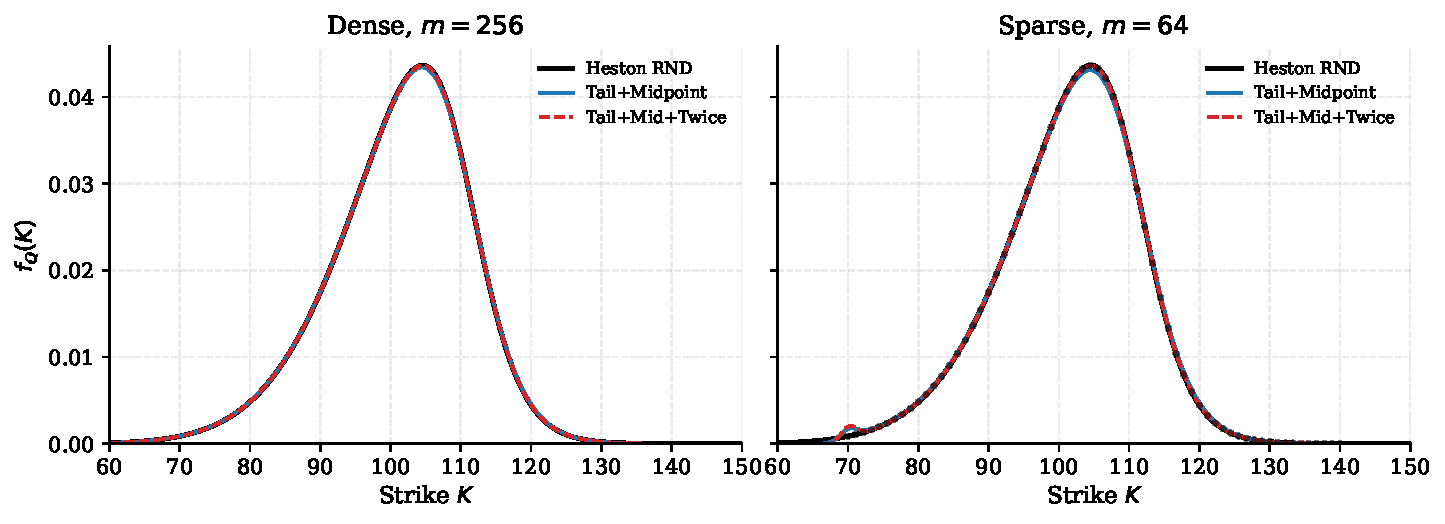
\includegraphics[width=0.98\textwidth]{figures_v2/ccdf_heston_rnd.pdf}
\caption{Heston density of \(S_T\) on \([60,150]\). Solid: Tail+Midpoint \eqref{eq:headline} at mesh \(h=1.2\delta\). Dashed: Tail+Mid+Twice \eqref{eq:twice}. Sparse quoted strikes are marked on the true density. Curves are truncated at zero.}
\label{fig:heston-rnd}
\end{figure}

On the dense chain \(K_1=30\) lies well to the left of the ISE window and \(C_m=0\); completing the tails does not change the baseline digits, and the mesh rule already matches that oracle (ratio \(1.02\)). Midpoints cut mesh ISE by a factor of thirty, to \(8.23\times 10^{-7}\) against an oracle \(2.27\times 10^{-7}\) (ratio \(3.6\)). Twicing then reaches mesh ISE \(5.00\times 10^{-9}\) against an oracle \(3.44\times 10^{-9}\) (ratio \(1.45\)), and is visually indistinguishable from the true density in Figure~\ref{fig:heston-rnd}. On the sparse chain \(K_1=70\) lies inside the window and \(P(K_1)=0.69\). Placing that mass at \(K_1\) makes the mesh rule unusable (ISE \(287\)). The left line \eqref{eq:left} with spacing equal to the quoted mesh brings c\`adl\`ag mesh ISE to \(6.34\times 10^{-5}\). Midpoints on the completed support are Tail+Midpoint: mesh ISE \(5.95\times 10^{-6}\) against oracle \(4.39\times 10^{-6}\) (ratio \(1.36\)). Twicing at the mesh \(h\) then reaches \(3.24\times 10^{-6}\) against an oracle \(2.07\times 10^{-6}\) (ratio \(1.56\)).

The density-scale rule \eqref{eq:h-den} is larger than the mesh on both chains (\(h=3.41\) on the dense grid, \(h=4.29\) on the sparse grid after the right wing). On exact dense quotes it oversmooths: twiced ISE \(8.24\times 10^{-6}\) against mesh \(5.00\times 10^{-9}\). On the sparse chain it is larger than both the twiced oracle and twicing at the mesh (\(3.09\times 10^{-5}\) against \(2.07\times 10^{-6}\) and \(3.24\times 10^{-6}\)). It is the rule used on listed chains in Section~\ref{sec:emp}, where the quotes are noisy.

Table~\ref{tab:vg-tail} repeats the design for the variance-gamma process of \citet{madan1998}. The process parameters are those of \citet{carrmadan1999}: \(\sigma=0.12\), \(\nu=0.2\), \(\theta=-0.14\). Spot, rate, dividend yield, and maturity are as above, as are the two strike grids and the ISE window. Variance gamma is a pure-jump L\'evy process. The true density of \(\log S_T\) is a modified Bessel function \citep{madan1998}; the density of \(S_T\) is that formula times \(1/K\). Calls are the discounted payoff of that density, evaluated by the trapezoid rule. There is no Monte Carlo noise.

\begin{table}[H]
\centering
\caption{Integrated squared error \(\int_{60}^{150}(\hat f_{\Q}-f_{\Q})^2\,\mathrm{d}K\) on exact variance-gamma quotes. Bandwidth columns as in Table~\ref{tab:heston-tail}.}
\label{tab:vg-tail}
\resizebox{\textwidth}{!}{%
\begin{tabular}{ll
  S[table-format=2.2]
  S[table-format=1.2e-1, scientific-notation=true]
  S[table-format=2.2]
  S[table-format=1.2e-1, scientific-notation=true]
  S[table-format=2.2]
  S[table-format=1.2e-1, scientific-notation=true]}
\toprule
\multicolumn{1}{c}{Chain} & \multicolumn{1}{c}{Estimator} &
  {\(h^{\ast}\)} & {Oracle ISE} & {Mesh \(h\)} & {Mesh ISE} & {Den.\ \(h\)} & {Den.\ ISE} \\
\midrule
Dense & Baseline \eqref{eq:fhat-Q}
  & 0.63 & 2.14e-4 & 0.89 & 2.42e-4 & 2.18 & 8.57e-4 \\
Dense & Tail completion
  & 0.63 & 2.14e-4 & 0.89 & 2.42e-4 & 2.18 & 8.57e-4 \\
Dense & Tail+Midpoint \eqref{eq:headline}
  & 0.54 & 1.69e-5 & 0.89 & 5.55e-5 & 2.18 & 7.18e-4 \\
Dense & Tail+Mid+Twice \eqref{eq:twice}
  & 0.63 & 2.88e-6 & 0.89 & 9.96e-6 & 2.18 & 2.18e-4 \\
\midrule
Sparse & Baseline \eqref{eq:fhat-Q}
  & 26.83 & 2.80e-2 & 1.33 & 2.87e2 & 2.88 & 2.86e1 \\
Sparse & Tail completion
  & 0.84 & 4.67e-4 & 1.33 & 5.66e-4 & 2.70 & 1.53e-3 \\
Sparse & Tail+Midpoint \eqref{eq:headline}
  & 0.84 & 5.23e-5 & 1.33 & 1.91e-4 & 2.70 & 1.26e-3 \\
Sparse & Tail+Mid+Twice \eqref{eq:twice}
  & 0.84 & 1.17e-5 & 1.33 & 4.45e-5 & 2.70 & 4.44e-4 \\
\bottomrule
\end{tabular}%
}
\end{table}

\begin{figure}[H]
\centering
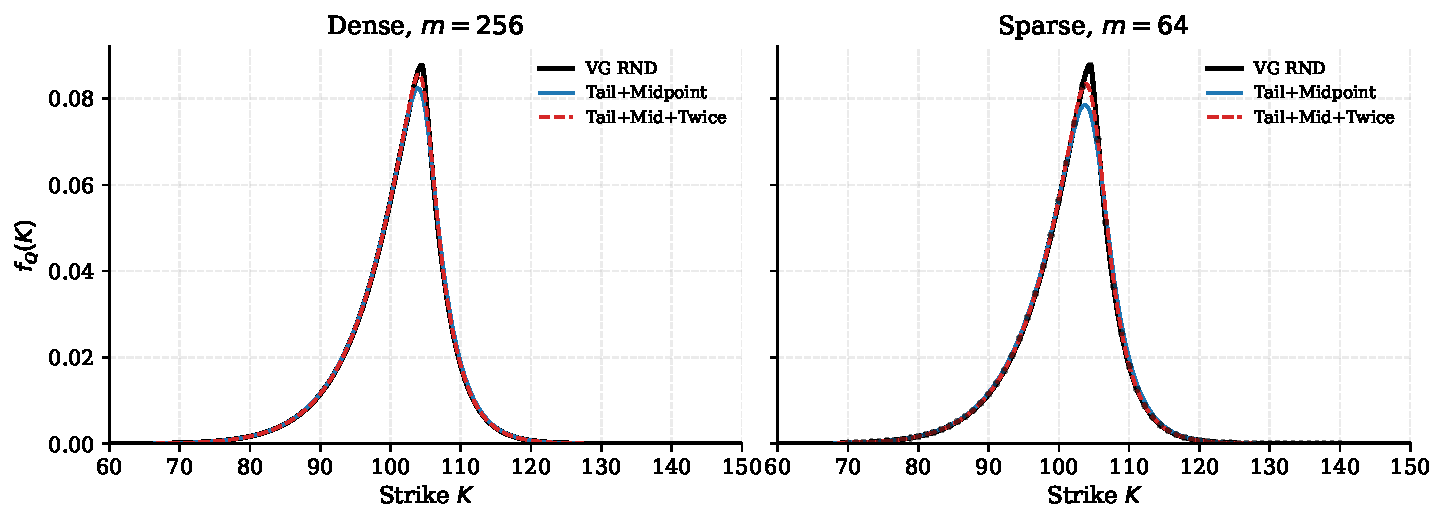
\includegraphics[width=0.98\textwidth]{figures_v2/ccdf_vg_rnd.pdf}
\caption{Variance-gamma density of \(S_T\) on \([60,150]\). Solid: Tail+Midpoint \eqref{eq:headline} at mesh \(h=1.2\delta\). Dashed: Tail+Mid+Twice \eqref{eq:twice}. Sparse quoted strikes are marked on the true density. Curves are truncated at zero.}
\label{fig:vg-rnd}
\end{figure}

On the dense chain the ranking is the same as under Heston. Completing the tails does not change the baseline digits. Midpoints cut mesh ISE from \(2.42\times 10^{-4}\) to \(5.55\times 10^{-5}\). Twicing then reaches \(9.96\times 10^{-6}\) against an oracle \(2.88\times 10^{-6}\) (ratio \(3.5\)), and tracks the peak in Figure~\ref{fig:vg-rnd}. The density of \(S_T\) is more peaked than under Heston, and the absolute errors are larger. On the sparse chain the c\`adl\`ag mesh rule is again unusable (ISE \(287\)). Tail+Midpoint mesh ISE is \(1.91\times 10^{-4}\); twicing at that \(h\) lowers it to \(4.45\times 10^{-5}\) against an oracle \(1.17\times 10^{-5}\). The density-scale rule oversmooths on both chains.

\section{Observation Noise}
\label{sec:noise}

The chains in Section~\ref{sec:ifc} are exact and equally spaced. A listed chain is neither. This section keeps the Heston and variance-gamma targets and changes the design in three ways. Strikes are irregular: twenty-two geometrically spaced knots on \([0.45F,0.90F)\), twenty-eight equally spaced knots on \([0.90F,1.10F)\), and twenty-two geometrically spaced knots on \([1.10F,1.40F]\), seventy-two strikes in all. The first strike lies inside the integrated-squared-error window \([60,140]\). Black--Scholes implied volatility is observed with independent Gaussian noise of standard deviation \(0.01\), then floored at \(0.02\), and converted back to a call. Thirty replications use the seed \(20260923\). Bandwidths and penalties are chosen without \(f_{\Q}\). The pilot mixture row is the exception: its constants minimize integrated squared error on the first eight replications.

Each fit is read twice. The density column is the formula \(\hat f_{\Q}\). The pricing column is the interpolant of the same fit. On the raw quotes, the density-scale rule \eqref{eq:h-den} is the bandwidth of the listed interpolant, and a second bandwidth is chosen by even/odd cross-validation of out-of-the-money pricing error. The two-step version builds a different call curve and then uses the same kernel at the density-scale bandwidth. The quoted calls are replaced by their Euclidean projection onto the decreasing convex cone with slopes in \([-e^{-rT},0]\), the quadratic program of Section~\ref{sec:emp}. Beyond the first and last strikes, implied volatility is held at its wing value and the calls are repriced on a log grid from \(0.15F\) to \(3F\). The mixture uses those same masses. It puts weight \(\alpha\) on the twiced Gaussian at bandwidth \(c h\) and weight \(1-\alpha\) on a sinc kernel at bandwidth \(s\cdot c h\), where \(h\) is the density-scale bandwidth of the training fold. The triple \((c,\alpha,s)\) is chosen by even/odd cross-validation of out-of-the-money pricing error on the grid \(c\in\{0.75,1,1.25,1.5\}\), \(\alpha\in\{\tfrac12,\tfrac34,1\}\), and \(s\in\{2,3\}\) when \(\alpha<1\). The pilot row freezes \(c=1\), \(\alpha=\tfrac12\), and \(s=3\), the triple with the lowest integrated squared error on the first eight replications of each design. Out-of-the-money premiums are floored at zero before the error is computed. The other methods are:

\begin{itemize}
\item \citeauthor{yatchew2006}, with the roughness penalty chosen by the same cross-validation. The unknown in the quadratic program is the call. Slope increments are not used: that map is ill-conditioned, and a sequential least-squares solver started from those increments stops on an infeasible subproblem and returns the isotonic start. In call coordinates the same program terminates at the projection. The fitted call is convex and decreasing, with slopes in \([-e^{-rT},0]\), so its second derivative is a discrete measure. It is scored on pricing error and not on integrated squared error.
\item \citeauthor{aitsahalia2003}: the same projection, then a local linear whose bandwidth is cross-validated, and a local cubic at \(0.9\,F\hat\sigma\sqrt{T}\,n^{-1/9}\) for the density.
\item \citeauthor{bondarenko2003}, forty-one lognormals on a uniform grid in log strike from the lowest quoted strike to the highest. The common width is cross-validated on a grid that starts at the center spacing. Weights are nonnegative. Sum-to-one and forward-mean conditions enter as penalties and the weights are not rescaled.
\item \citeauthor{priestley1972}, the cubic of Section~\ref{sec:naive}, at two bandwidths: the cross-validated pricing bandwidth, and \(1.06\,F\hat\sigma_{\mathrm{ATM}}\sqrt{T}\,n^{-1/9}\).
\item A raw SVI slice \citep{gatheral2006}. Total implied variance is \(a+b\bigl(\rho(k-m)+\sqrt{(k-m)^2+\sigma^2}\bigr)\), fitted to call prices by least squares. The butterfly function \(g(k)\) of \citet{gatheraljacquier2014} is penalized wherever it is negative.
\end{itemize}

Integrated squared error uses the density formula, \(\int_{60}^{140}(\hat f_{\Q}-f_{\Q})^2\,\mathrm{d}K\). The pricing column uses the interpolant, the kernel cdf clipped to \([0,1]\), and is out-of-the-money root-mean-square error against the clean calls. The two columns are not two summaries of one function.

\begin{table}[H]
\centering
\caption{Noisy irregular grids, thirty replications. The first line of each method is the mean and the second is the replication standard deviation. Columns \(\hat f_{\Q}\) are integrated squared error of the density formula. Columns \(\hat P\) are out-of-the-money pricing error of the interpolant against the clean calls. Yatchew--H\"ardle has no density formula.}
\label{tab:noise}
\resizebox{\textwidth}{!}{%
\begin{tabular}{ll *{4}{S[table-format=1.2e-1,scientific-notation=true]}}
\toprule
& & \multicolumn{2}{c}{Heston} & \multicolumn{2}{c}{Variance gamma} \\
\cmidrule(lr){3-4} \cmidrule(lr){5-6}
Method & Rule & {$\hat f_{\Q}$} & {$\hat P$} & {$\hat f_{\Q}$} & {$\hat P$} \\
\midrule
Mixture & pricing CV
  & 6.62e-4 & 3.21e-2 & 4.23e-3 & 3.49e-2 \\
 & & 8.76e-4 & 1.12e-2 & 3.57e-3 & 8.70e-3 \\
\addlinespace
Mixture & pilot, \(\alpha=\tfrac12\), \(3h\)
  & 2.79e-4 & 3.08e-2 & 1.27e-3 & 2.94e-2 \\
 & & 1.31e-4 & 8.20e-3 & 5.52e-4 & 7.80e-3 \\
\addlinespace
Two-step & projection, flat wing
  & 4.29e-4 & 2.91e-2 & 2.35e-3 & 3.17e-2 \\
 & & 2.63e-4 & 9.10e-3 & 1.34e-3 & 8.00e-3 \\
\addlinespace
Kernel & density scale
  & 5.72e-3 & 3.68e-2 & 8.94e-2 & 4.22e-2 \\
 & & 7.59e-3 & 1.36e-2 & 1.15e-1 & 1.40e-2 \\
\addlinespace
Kernel & pricing CV
  & 7.72e-2 & 3.82e-2 & 1.49e-1 & 4.02e-2 \\
 & & 2.61e-1 & 1.51e-2 & 6.05e-1 & 1.09e-2 \\
\addlinespace
Yatchew--H\"ardle & CV penalty
  & {---} & 4.22e-2 & {---} & 4.16e-2 \\
 & & {---} & 9.29e-3 & {---} & 9.25e-3 \\
\addlinespace
A\"{\i}t-Sahalia--Duarte & CV / \(n^{-1/9}\)
  & 4.67e-4 & 4.31e-2 & 2.01e-3 & 3.81e-2 \\
 & & 1.18e-4 & 1.19e-2 & 6.20e-4 & 1.08e-2 \\
\addlinespace
PCA & CV width
  & 8.11e-4 & 3.29e-2 & 1.70e-3 & 3.76e-2 \\
 & & 1.34e-3 & 9.97e-3 & 9.92e-4 & 1.77e-2 \\
\addlinespace
Priestley--Chao & pricing CV
  & 2.51e-2 & 4.50e-2 & 1.85e-2 & 4.16e-2 \\
 & & 1.50e-2 & 1.10e-2 & 1.28e-2 & 1.51e-2 \\
\addlinespace
Priestley--Chao & \(n^{-1/9}\)
  & 8.92e-4 & 4.34e-1 & 3.14e-3 & 2.34e-1 \\
 & & 1.46e-4 & 3.15e-2 & 6.52e-4 & 2.95e-2 \\
\addlinespace
SVI & price fit
  & 2.46e-3 & 2.86e-2 & 2.26e-2 & 2.87e-2 \\
 & & 4.95e-3 & 1.05e-2 & 2.61e-2 & 8.07e-3 \\
\bottomrule
\end{tabular}%
}
\end{table}

\begin{figure}[H]
\centering
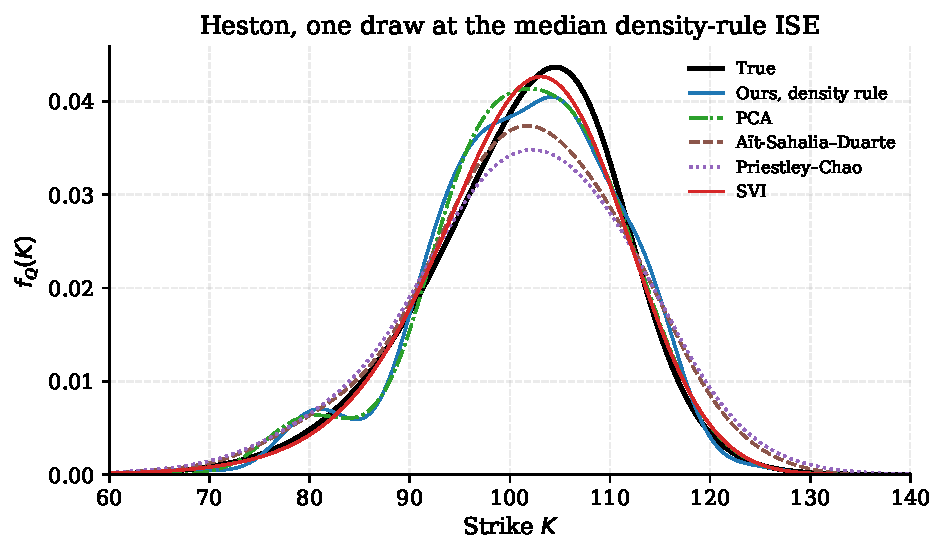
\includegraphics[width=0.92\textwidth]{figures_v2/noise_heston.pdf}
\caption{One Heston draw, the replication whose density-scale integrated squared error is the sample median. Curves other than the truth are truncated at zero for display. Priestley--Chao is shown at the second-derivative bandwidth.}
\label{fig:noise-heston}
\end{figure}

\begin{figure}[H]
\centering
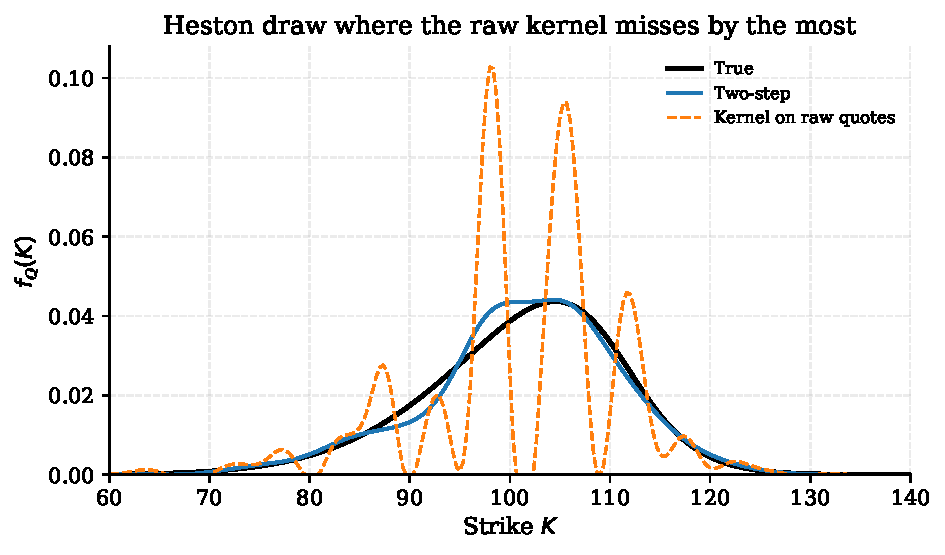
\includegraphics[width=0.92\textwidth]{figures_v2/noise_twostep.pdf}
\caption{The Heston replication in which the raw kernel's integrated squared error exceeds the two-step estimator by the most: \(0.025\) against \(2.9\times 10^{-4}\). Curves are truncated at zero for display.}
\label{fig:twostep}
\end{figure}

On the raw quotes the local cubic and the retuned convolution are closer to \(f_{\Q}\) than the density-scale kernel. Cross-validating that kernel on pricing error makes the density worse: under Heston the mean integrated squared error rises from \(5.7\times 10^{-3}\) to \(7.7\times 10^{-2}\). The second-derivative Priestley--Chao bandwidth has Heston pricing error \(0.43\); the same cubic at a pricing bandwidth has pricing error \(0.045\) and a worse density.

Projecting the calls and holding the wings at the wing implied volatility is the step that removes the arbitrage noise in the jumps. The twiced Gaussian on that curve has mean integrated squared error \(4.3\times 10^{-4}\) under Heston, below the local polynomial (\(4.7\times 10^{-4}\)) and the convolution (\(8.1\times 10^{-4}\)), and \(2.3\times 10^{-3}\) under variance gamma, above both. Figure~\ref{fig:twostep} is the Heston draw on which the raw kernel is worst: integrated squared error \(0.025\), against \(2.9\times 10^{-4}\) once the same kernel is applied to the projected call.

Moving half of that kernel onto a sinc at three times the bandwidth, with the constants chosen by integrated squared error on the first eight replications, lowers the thirty-replication means to \(2.8\times 10^{-4}\) and \(1.3\times 10^{-3}\). That is the smallest integrated squared error in Table~\ref{tab:noise}, on both targets, and the clean-call error is \(0.031\) and \(0.029\) against \(0.029\) for SVI. Those two constants see the true density on the pilot.

Pricing cross-validation of \((c,\alpha,s)\), run after the projection and the wing, uses held-out quotes. The modal Heston choice is \(c=1.25\), \(\alpha=\tfrac12\), \(s=2\) (nine of thirty draws). The mean integrated squared error rises to \(6.6\times 10^{-4}\) under Heston and \(4.2\times 10^{-3}\) under variance gamma. The Heston median is \(4.0\times 10^{-4}\). Under Heston that row still beats the convolution. Under variance gamma it beats neither the convolution nor the local polynomial. It does not recover the pilot pair, and Section~\ref{sec:emp} does not use it. Listed prices are the interpolant of the density-scale kernel and of the two-step Gaussian.

\section{Empirical Illustration}
\label{sec:emp}

\subsection{Data}
\label{sec:data}

Four slices illustrate the estimator. They are not a panel. The S\&P~500 snapshot is 6~September 2026, 17:04 Eastern; the Nasdaq-100 snapshot is 8~September 2026, 17:17 Eastern; the Russell~2000 snapshot is 19~September 2026, 03:44 Eastern, outside the cash session. Only the standard monthly roots are kept. Time to expiry is \(T=d/365.25\). The discount rate is a flat \(r=0.04\), and the forward is the median of \(K+e^{rT}(C-P)\) near the money, so an error in \(r\) moves \(F\). The quote filter is unchanged: a positive bid, ask at least the bid, mid at least \(0.25\), and spread at most \(\max(15,0.5\times\mathrm{mid})\). Out-of-the-money mids are kept and the other side is filled by parity. Puts with \(K<0.7F\) and mid below \(0.50\) are dropped. Table~\ref{tab:data} records the counts.

The December 2026 S\&P~500 strip (\(T=0.282\), \(S_0=7718.60\), \(F=7786\), \(q=0.92\%\)) has \(393\) strikes on \([0.31F,1.36F]\) after the screens. The March 2027 strip (\(T=0.531\), \(F=7864\)) has \(222\). The Nasdaq-100 December strip (\(T=0.277\), \(F=29898\)) has \(252\). The Russell~2000 December strip (\(T=0.246\), \(F=2883\)) has \(97\). Density-scale bandwidths are \(h=180\), \(291\), \(1082\), and \(97.8\).

\begin{table}[H]
\centering
\caption{Construction of the working slices. ``At expiry'' counts listed puts and calls on that root and maturity with a positive bid and ask at least the bid. ``Screens'' applies the mid and spread filters. ``Working OTM'' is the slice used by the estimators.}
\label{tab:data}
{\small
\begin{tabular}{@{}l *{5}{S[table-format=3.0]}@{}}
\toprule
\multicolumn{1}{@{}c}{Slice} & {At expiry} & {Screens} & {Unique \(K\)} & {Working OTM} & {Puts} \\
\midrule
SPX 18 Dec 2026 & 819 & 812 & 416 & 393 & 303 \\
SPX 19 Mar 2027 & 453 & 452 & 228 & 222 & 164 \\
NDX 18 Dec 2026 & 555 & 531 & 279 & 252 & 185 \\
RUT 18 Dec 2026 & 217 & 216 & 115 & 97 & 56 \\
\bottomrule
\end{tabular}
}
\end{table}

\subsection{The interpolant}
\label{sec:emp-est}

This section prices with the interpolant. It does not integrate \(\hat f_{\Q}\). For the kernel, the price is the cdf readout at the density-scale bandwidth: \(\hat P\) clipped to \([0,1]\), and \(C=S_0e^{-qT}(1-\hat P)\). The two-step row is the same readout after the projection and the flat wing of Section~\ref{sec:noise}. Hold-out refits that pipeline on each even/odd half and scores the other half. Premiums are floored at zero. The competitors contribute their own call fits, not a second derivative.

\begin{table}[H]
\centering
\caption{Listed slices, interpolant only. Entries are out-of-the-money root-mean-square error in index points. Hold-out refits on each even/odd half. Nothing in this table is an integral of \(\hat f_{\Q}\).}
\label{tab:listed}
\begin{tabular}{ll *{2}{S[table-format=1.2e-1,scientific-notation=true]}}
\toprule
Slice & Method & {In sample} & {Hold-out} \\
\midrule
SPX Dec & Interpolant & 4.88e-1 & 9.46e-1 \\
 & Two-step interpolant & 4.99e-1 & 8.69e-1 \\
 & Yatchew--H\"ardle & 2.20e-2 & 5.40e-2 \\
 & A\"{\i}t-Sahalia--Duarte & 4.11e-1 & 5.40e-1 \\
 & PCA & 3.96e-2 & 4.28e-2 \\
 & Priestley--Chao & 9.08e-2 & 3.48e-1 \\
 & SVI & 5.32e-1 & 5.32e-1 \\
\midrule
SPX Mar & Interpolant & 9.55e-1 & 1.90e0 \\
 & Two-step interpolant & 9.40e-1 & 1.72e0 \\
 & Yatchew--H\"ardle & 3.80e-2 & 1.41e-1 \\
 & A\"{\i}t-Sahalia--Duarte & 6.51e-1 & 8.61e-1 \\
 & PCA & 8.73e-2 & 1.02e-1 \\
 & Priestley--Chao & 3.22e-1 & 1.28e0 \\
 & SVI & 1.16e0 & 1.16e0 \\
\midrule
NDX Dec & Interpolant & 6.45e0 & 8.74e0 \\
 & Two-step interpolant & 6.42e0 & 8.82e0 \\
 & Yatchew--H\"ardle & 2.06e0 & 3.05e0 \\
 & A\"{\i}t-Sahalia--Duarte & 3.72e0 & 4.73e0 \\
 & PCA & 2.93e0 & 3.23e0 \\
 & Priestley--Chao & 2.88e0 & 7.41e0 \\
 & SVI & 3.12e0 & 3.29e0 \\
\midrule
RUT Dec & Interpolant & 4.03e-1 & 9.64e-1 \\
 & Two-step interpolant & 4.46e-1 & 8.14e-1 \\
 & Yatchew--H\"ardle & 2.30e-2 & 1.55e-1 \\
 & A\"{\i}t-Sahalia--Duarte & 3.60e-1 & 4.94e-1 \\
 & PCA & 2.92e-2 & 3.29e-2 \\
 & Priestley--Chao & 2.11e-1 & 8.36e-1 \\
 & SVI & 1.17e-1 & 1.17e-1 \\
\bottomrule
\end{tabular}
\end{table}

On these four slices the interpolant and the two-step interpolant are close. The quotes already lie near the decreasing convex cone, so the projection moves them by hundredths of an index point and the density-scale bandwidth smooths either curve the same way. December S\&P~500 error is \(0.49\) for the interpolant and \(0.50\) for the two-step interpolant, with hold-out \(0.95\) and \(0.87\). March is \(0.96\) and \(0.94\). The Nasdaq-100 strip is \(6.45\) and \(6.42\). The Russell~2000 strip is \(0.40\) and \(0.45\).

The convex projection is the closest of these methods to the quotes. On the December S\&P~500 strip its in-sample error is \(0.022\) and its hold-out error is \(0.054\). The cross-validated penalty is \(1\) in the normalized units of Section~\ref{sec:noise}. A pure interpolating projection is available, and the hold-out selects the penalized fit. The same pattern holds on the other three slices (penalties \(1\), \(0.1\), and \(10\)). The quotes are close to the decreasing convex cone once the quadratic program is solved in the call. An earlier implementation, parameterized by slope increments, stopped with an infeasible subproblem and returned an isotonic start whose December S\&P~500 residual was about \(2.25\). The distance to the cone is the solved residual above.

The positive convolution, with centers on the quoted log-strike range and a width at the bottom of the cross-validation grid, is the next pricing method on every slice. December S\&P~500 error is \(0.040\) in sample and \(0.043\) on hold-out. On the Russell~2000 strip the hold-out errors are \(0.033\) for the convolution and \(0.155\) for the projection. SVI prices the December strip at \(0.53\) and the Russell~2000 strip at \(0.12\). Its butterfly function is nonnegative on the monitoring grid, up to a solver tolerance of \(3\times 10^{-7}\) on the March S\&P~500 strip.

The local polynomial starts from the solved projection. On the December S\&P~500 strip its error is \(0.41\) in sample and \(0.54\) on hold-out. Hold-out error exceeds in-sample error on every slice. Priestley--Chao at its pricing bandwidth has December error \(0.091\) and Nasdaq-100 error \(2.88\). Figure~\ref{fig:listed} is the other readout of the same kernel: the density formula on the December slices. Table~\ref{tab:listed} scores the interpolant.

\begin{figure}[H]
\centering
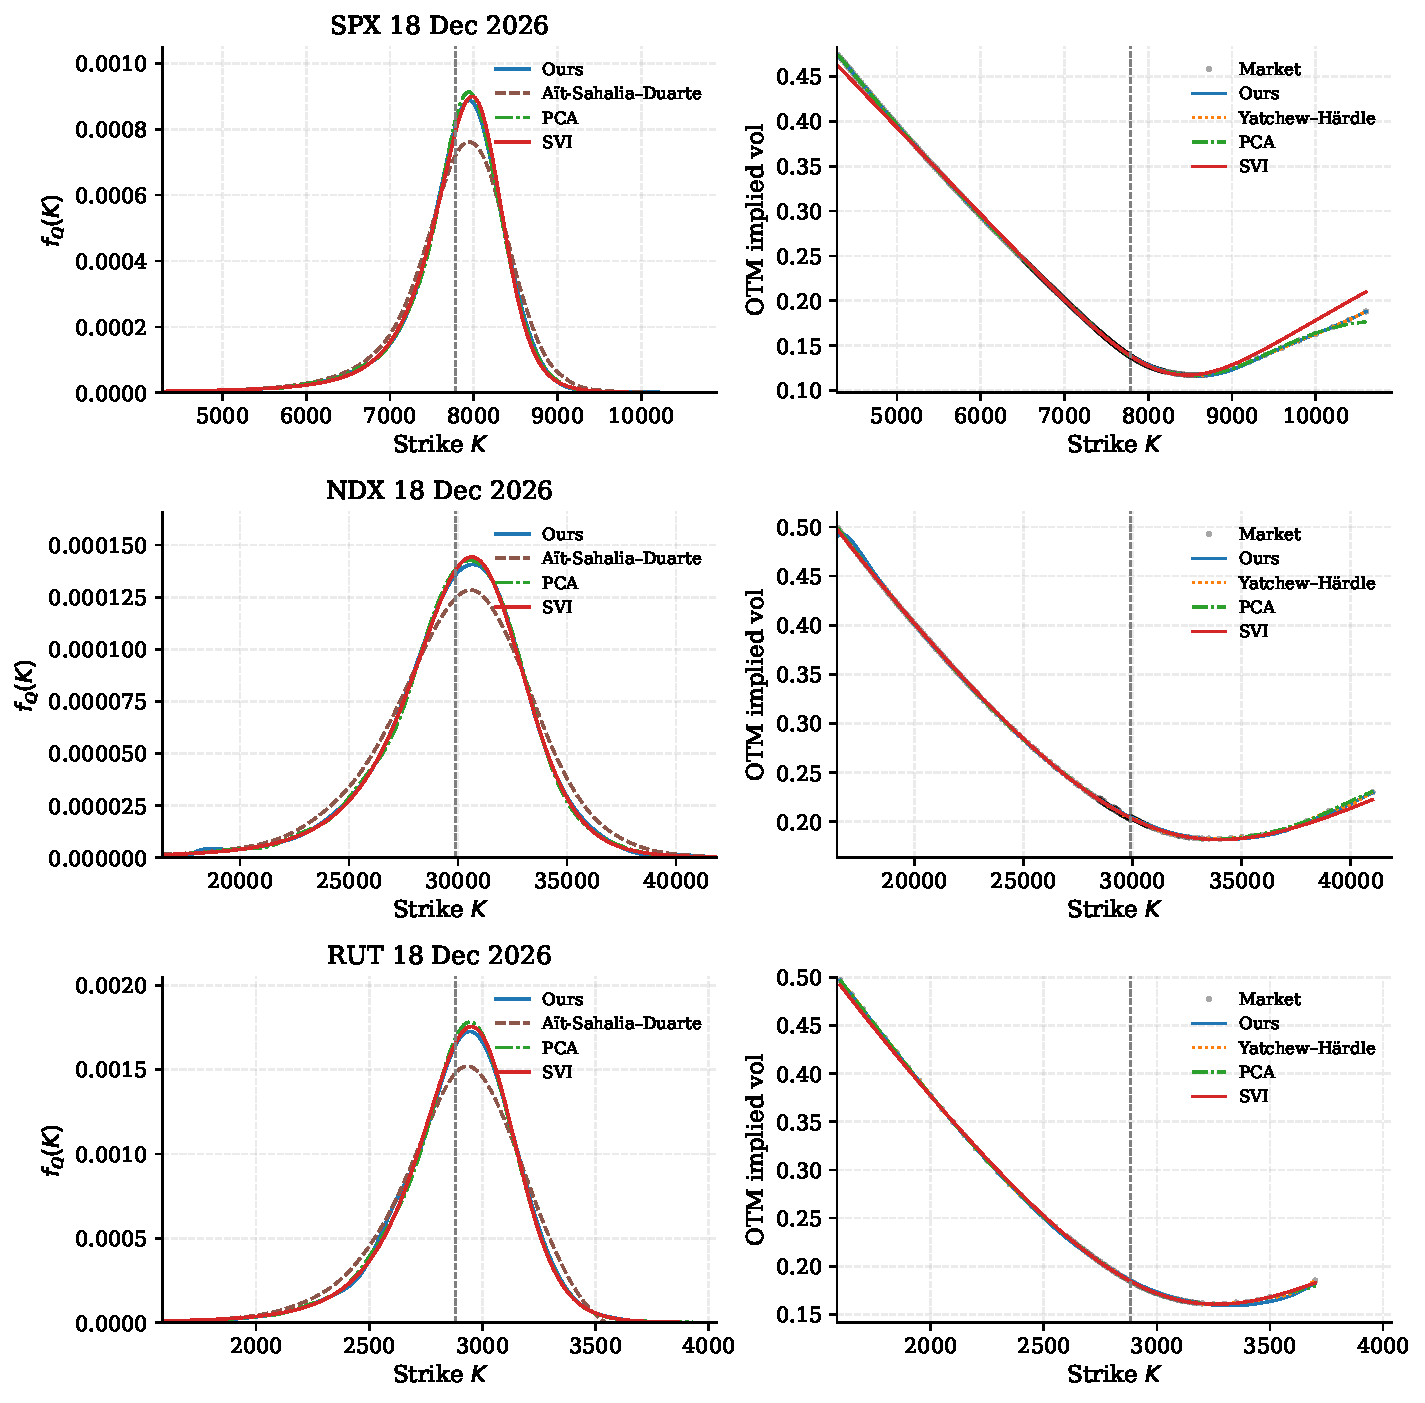
\includegraphics[width=0.98\textwidth]{figures_v2/ccdf_listed.pdf}
\caption{December 2026 slices. Left: the density formula, positive part, with the local cubic, the convolution, and SVI. Right: out-of-the-money implied volatility of the listed quotes. The dashed line is the forward. Table~\ref{tab:listed} scores the kernel cdf of the same estimator.}
\label{fig:listed}
\end{figure}

\section{Conclusion}
\label{sec:conc}

The second strike derivative of a European call is the risk-neutral density of the underlying at expiry. On a finite strike list that derivative is not an estimator. Rescaling the calls to a complementary distribution function makes the object to be smoothed a jump measure. A Gaussian kernel then has a closed form. The density formula is minus the forward times the derivative of the kernel density of those jumps. The call interpolant is the kernel cdf, clipped to \([0,1]\). Completing the tails, placing masses at cell centers, and combining two widths are quadrature corrections. On exact equally spaced Heston quotes the density formula brings the integrated squared error to \(5.0\times 10^{-9}\). The same ordering holds for variance gamma.

Over the whole line the signed density integrates to zero and its first moment equals the forward, before and after twicing. Prices are read from the clipped cdf.

On noisy irregular strikes the jumps of the raw call are the wrong measure. Projecting the calls onto the decreasing convex cone and holding the wings at the wing implied volatility, then applying the twiced Gaussian, lowers the Heston mean integrated squared error to \(4.3\times 10^{-4}\), below the local polynomial and the convolution, and the variance-gamma mean to \(2.3\times 10^{-3}\), above both. The pricing column of that comparison is the interpolant of the same fit. An equal Gaussian--sinc mixture with the sinc at three times the bandwidth reaches \(2.8\times 10^{-4}\) and \(1.3\times 10^{-3}\), with those constants chosen by integrated squared error on eight pilot replications. Pricing cross-validation of the same constants does not recover that pair. Section~\ref{sec:emp} prices with the interpolant of the twiced Gaussian, at the density-scale bandwidth, on the raw quotes and on the projected curve.

On the four listed slices those two interpolants are close to each other and well above the unsmoothed projection. December S\&P~500 error is \(0.49\) for the interpolant and \(0.022\) for the projection. The projection's second derivative is a discrete measure. The density formula remains the readout for \(f_{\Q}\).

\section*{Code and Data Availability}
A Python implementation of \eqref{eq:twice} and the replication scripts are available at \url{https://github.com/s-broda/RND}.
The v2 comparison is \path{python/replicate_v2.py}.
The two-step estimator is \path{python/src/twostep.py}.

\bibliographystyle{elsarticle-harv}
\bibliography{refs_v2}
\end{document}
